\documentclass[tikz,border=10pt]{standalone}
\usetikzlibrary{calc}

\begin{document}
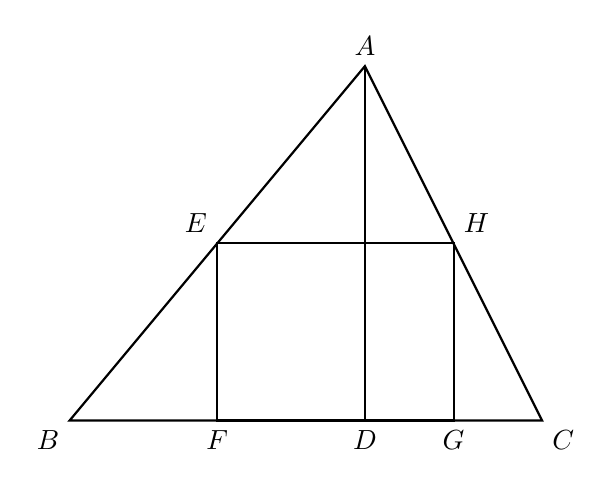
\begin{tikzpicture}[scale=1.5,thick]
    % 1. 定义三角形的基本坐标
    \coordinate (B) at (0,0);
    \coordinate (C) at (4,0);
    \coordinate (A) at (2.5,3); % 顶点A位置
    
    % 2. 绘制三角形主体
    \draw (A) -- (B) -- (C) -- cycle;
    
    % 3. 定义高 AD
    \coordinate (D) at (2.5,0); % AD 垂足
    \draw (A) -- (D);
    
    % 4. 定义矩形 EFGH 上层顶点 (设定比例以符合视觉效果)
    % 设 E 为 AB 上的点，H 为 AC 上的点，使 EH || BC
    % 这里选取高度 y=1作为矩形顶部
    \def\h{1.5}
    \path let \p1 = (A), \p2 = (B), \p3 = (C) in
        coordinate (E) at ($(B)!{1-\h/3}!(A)$)  % E 在 AB 上
        coordinate (H) at ($(C)!{1-\h/3}!(A)$); % H 在 AC 上
    
    % 5. 投影点 F 和 G
    \coordinate (F) at (E |- B);
    \coordinate (G) at (H |- B);
    
    % 6. 绘制矩形 EFGH
    \draw (E) rectangle (G);
    
    % 7. 标注所有点
    \node[below left]  at (B) {$B$};
    \node[below right] at (C) {$C$};
    \node[above]       at (A) {$A$};
    \node[below]       at (D) {$D$};
    \node[below]       at (F) {$F$};
    \node[below]       at (G) {$G$};
    \node[above left]  at (E) {$E$};
    \node[above right] at (H) {$H$};

\end{tikzpicture}
\end{document}